\documentclass{article}
\usepackage{indentfirst}
\usepackage[pdftex]{graphicx}
\usepackage{graphicx}
\usepackage{picture}
\usepackage{graphics}
\usepackage{hyperref}
\usepackage{amsmath} % for argmax
\usepackage{bm} % used for bolding the equation
\title{91.542 - Natural Language Processing ~\\ Homework Assignmen 3}
\author{Chang Liu ~\\ chang\_liu@student.uml.edu}


\begin{document}
\maketitle


\section{Problem 1. [20 pts] Huffman code}

\textbf{Answer:}~\\
(1) The building process of the huffman code is as follows:

\begin{center}
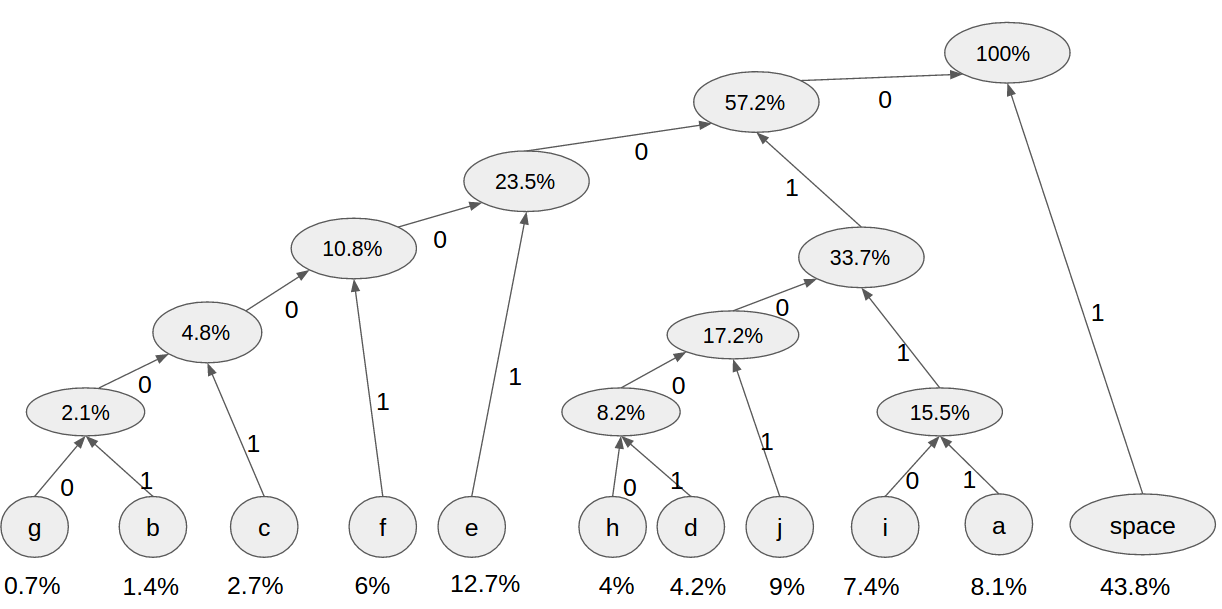
\includegraphics[scale=0.3]{hw3_fig1.png}
\end{center}

The basic algorithm is to sort the nodes from low to high, and merge each two elements with the lowest frequency into one node, and then do it iteratively to connect all the nodes. After that, mark the left route as `0' and right path as `1'. At last, the huffman code for each symbol is represented by visiting the nodes and listing all the numbers in the path.~\\


(2) The word ``headi'' is consist of five different symbols, which is `h', `e', `a', `d', `i', we just need to get its code correspondingly and then concanate them, which is `01000', `001', `0111', `01001', `0110'. So the overall representation is `010000010111010010110'. ~\\

(3) First we can build a table that represents all the symbols, representations and its length, as follows:

\begin{center}
    \begin{tabular}{| l | l | l |}
    \hline
    Symbol & Representation & Length \\ \hline
    a & 0111 & 4 \\ \hline
    b & 000001 & 6 \\ \hline
    c & 00001 & 5 \\ \hline
    d & 01001 & 5 \\ \hline
    e & 001 & 3 \\ \hline
    f & 0001 & 4 \\ \hline
    g & 000000 & 6 \\ \hline
    h & 01000 & 5 \\ \hline
    i & 0110 & 4 \\ \hline
    j & 0101 & 4 \\ \hline
    space & 1 & 1 \\ \hline
    \end{tabular}
\end{center}

So the average value is:
$$ \frac{4+6+5+5+3+4+6+5+4+4+1}{11} = \frac{47}{11} \approx 4.27$$

(4) For entropy, use the following equation and the probability in the table from the question description, we can get the value:
\begin{flalign*}
H(p) &= H(X) \\
&= - \sum_{x \in X}{p(x) \log_2{p(x)}} \\
&= - (8.1\% * \log_2{8.1\%} + 1.4\% * \log_2{1.4\%} + ... + 43.8\% * \log_2{43.8\%}) \\
&\approx 2.68 
\end{flalign*}


\section{Problem 2. [30 pts] Evaluating a clustering solution}

\textbf{Answer:} ~\\

(1) According to following equation, we can know the entropy of a clustering solution:

$$ Entropy(C,S)  = \sum_{i}{\frac{|c_i|}{n} \sum_{j}{\frac{|c_i \bigcap s_j|}{|c_i|} \log{\frac{|c_i \bigcap s_j|}{|c_i|}}}}$$

In the equation, $c_i$ is a cluster from $C$, and $s_j$ is a cluster from solution $S$, so we can get the entropy as follows:

\begin{flalign*}
entropy &= \sum_{i \in C}{\frac{|c_i|}{n} \sum_{j \in S}{\frac{|c_i \bigcap s_j|}{|c_i|} \log{\frac{|c_i \bigcap s_j|}{|c_i|}}}} \\
&= \frac{1}{10} * [(\frac{2}{4} * \log_2{\frac{2}{4}} * 2 + 0 + 0) * 4 + (0 + \frac{1}{3} * \log_2{\frac{1}{3}} +\frac{2}{3} * \log_2{\frac{2}{3}} + 0 ) * 3 \\
&+ (0 + \frac{1}{2} * \log_2{\frac{1}{2}} * 2 + 0) * 2 + (\frac{1}{1} * \log_2{\frac{1}{1}} + 0 + 0 + 0) * 1] \\
&\approx -0.88
\end{flalign*}

Regarding the entropy, we have to get the negative value of the above equation, which should be \underline{\textbf{0.88}}

Similarly, we can get the second clustering solutions, as follows:

\begin{flalign*}
entropy &= \sum_{i \in C}{\frac{|c_i|}{n} \sum_{j \in S}{\frac{|c_i \bigcap s_j|}{|c_i|} \log{\frac{|c_i \bigcap s_j|}{|c_i|}}}} \\
&= \frac{1}{10} * [ 4 * (\frac{3}{4} * \log_2{\frac{3}{4}} + \frac{1}{4} * \log_2{\frac{1}{4}})  + 3 * (\frac{2}{3} * \log_2{\frac{2}{3}} + \frac{1}{3} * \log_2{\frac{1}{3}}) \\
&+ 3 * (\frac{1}{3} * \log_2{\frac{1}{3}} * 3)] \\
&\approx -1.08
\end{flalign*}

So for the second clustering solution, the entropy is \underline{\textbf{1.08}}


(2) First, we can get the equation as follows:

$$ Bcubed \quad  Precision = \frac{\sum_{e}{\frac{|c_e \bigcap s_e|}{|c_e|}}}{n}$$
$$ Bcubed \quad  Recall = \frac{\sum_{e}{\frac{|c_e \bigcap s_e|}{|s_e|}}}{n}$$

For the first solution, the BCubed precision and recall is as follows:

\begin{flalign*}
Bcubed-precision &= \frac{\frac{2}{4} + \frac{2}{4} + \frac{1}{1} + \frac{2}{4} + \frac{2}{4} + \frac{1}{3} + \frac{1}{2} + \frac{2}{3} + \frac{2}{3} + \frac{1}{2}}{10} \\
&= \frac{17}{30} \\
&\approx 56.67\% \\
Bcubed-recall &= \frac{\frac{2}{3} + \frac{2}{3} + \frac{1}{3} + \frac{2}{4} + \frac{2}{4} + \frac{1}{4} + \frac{1}{4} + \frac{2}{2} + \frac{2}{2} + \frac{1}{1}}{10} \\
&= \frac{37}{60} \\
&\approx 61.67\% \\
F1-score &= 2 * \frac{P * R}{P + R} \\
&= 2 * \frac{\frac{17}{30} * \frac{37}{60}}{\frac{17}{30} + \frac{37}{60}} \\
&\approx 0.59
\end{flalign*}

For the second solution, similarly we can calculate the value, the BCubed precision and recall is as follows:
\begin{equation*}
Bcubed-precision \approx 51.67\%, ~\\
Bcubed-reall = 65\%, ~\\
F1-score \approx 0.58
\end{equation*}

(3) The first system is better, since it has less entropy, according to the entropy measure.

(4) The first system is better, since it has higher F1-score.

\section{Problem 3. [10 pts] Leave-one-out (LOO) cross-validation}


\section{Problem 4. [50 pts] Computing similarity}

\end{document}